\documentclass[tikz,border=10pt]{standalone}
\usepackage{tikz}
\usetikzlibrary{calc}

\begin{document}
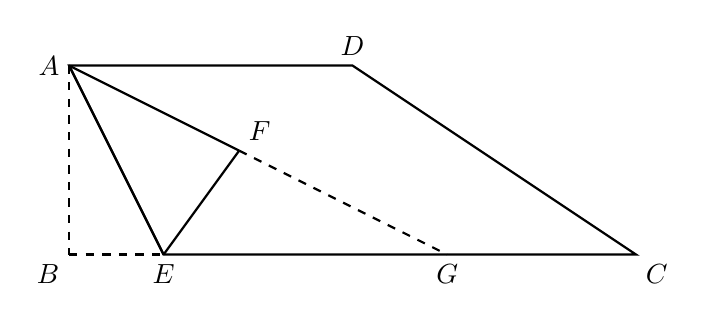
\begin{tikzpicture}[scale=1.2, >=stealth]
    % --- 1. 定义坐标点 ---
    % 设 A 为原点上方点，根据视觉比例设定参数
    \coordinate (A) at (0, 2);
    \coordinate (B) at (0, 0);
    \coordinate (D) at (3, 2);
    \coordinate (C) at (6, 0);

    % E点在BC上，设定翻折位置
    \coordinate (E) at (1, 0);

    % 计算 F 点：B 关于 AE 的对称点
    % 根据翻折性质，F 点在以 A 为圆心，AB 为半径的圆上
    % 这里根据原图 A,F,G 共线的视觉特征进行定位
    \coordinate (F) at (1.8, 1.1); % 约略位置，满足几何示意

    % G 点在 BC 上，且 A, F, G 三点共线
    % 使用 TikZ 的计算交点功能或比例延伸
    \coordinate (G) at (intersection of A--F and B--C);

    % --- 2. 绘制图形边界与线段 ---
    % 绘制实线部分
    \draw[thick] (A) -- (D) -- (C) -- (E) -- cycle;
    \draw[thick] (A) -- (E);
    \draw[thick] (E) -- (F);

    % 绘制虚线部分 (表示原始边或辅助线)
    \draw[dashed, thick] (A) -- (B);
    \draw[dashed, thick] (B) -- (E);
    \draw[dashed, thick] (F) -- (G);
    \draw[thick] (A) -- (F); % 事实上 A-F-G 是一条线

    % --- 3. 标注文本 ---
    \node[left] at (A) {$A$};
    \node[below left] at (B) {$B$};
    \node[below] at (E) {$E$};
    \node[below] at (G) {$G$};
    \node[below right] at (C) {$C$};
    \node[above] at (D) {$D$};
    \node[above right] at (F) {$F$};

    % --- 4. 绘制直角标记 (可选，增加学术专业度) ---
    % 如果需要体现 F 是直角，可以取消下面代码的注释
    % \draw ($(F)!0.2!(E)$) -- ($(F)!0.2!(E)+(F)!0.2!(A)-(F)$)--($(F)!0.2!(A)$);

\end{tikzpicture}
\end{document}